\section{Auswertung}
\subsection{Fourier-Analyse}
Zunächst wird mit der Gleichung (\ref{eq:2}) die Amplituden für die unterschiedlichen
Schwingungsformen bestimmt.\\
\centerline{\textbf{Rechteckspannung}}
Die Funtkion ist ungerade, damit fällt bei der Gleichung (\ref{eq:1}) $a_n$ weg.
Somit kann für die Berechnung der Amplitude die Form $b_n$ nehmen.
\begin{equation*}
  \text{Für $f(t)$ gilt:}
  \begin{cases}
    A \, \text{für} \, 0 \leq t \leq \frac{T}{2} \\
    -A \, \text{für} \, -\frac{T}{2} \leq t \leq 0
  \end{cases}
\end{equation*}
Damit ist
\begin{align*}
  b_n &= -\frac{2}{T} [(-A \int_{-\frac{T}{2}}^0 sin(\frac{2\pi nt}{T})dt) + (A \int_0^{\frac{T}{2}} sin(\frac{2\pi nt}{T})dt))]\\
\implies b_n &=\frac{2A}{T} (\frac{T}{2\pi n}(1-cos(\pi))\\
\implies b_n &= \frac{2A}{\pi n}(1-(-1)^n)
\end{align*}
Nun folgt, dass für
\begin{equation*}
  \text{n}
  \begin{cases}
    gerade \implies b_n = 0 \,\, \\
    ungerade \implies b_n = \frac{4A}{\pi n}
  \end{cases}
\end{equation*}
Somit lautet die Funktion $f(t) = \sum^{\infty}_{n=1} \frac{4A}{\pi (2n-1)} \cdot sin(\frac{2\pi}{T}\cdot(2n-1)t)$.
\begin{table}[H]
  \centering
  \begin{tabular}{c c c c}
    \toprule\\
    Anzahl & $A_{mess} / V$ & $A_{theo} / V$ & $Abweichung / \% $\\
    \midrule \\
    1 & 1070 & 1070 & 0 \\
    2 & 656  & 681 & 3,67\\
    3 & 440  & 454 & 3,08\\
    4 & 320  & 340 & 5,88\\
    5 & 288  & 272 & 5.88\\
    6 & 252  & 227 & 11,01\\
    7 & 208  & 194 & 7,22\\
    8 & 160  & 170 & 5,88\\
    9 & 158  & 151 & 4,64\\
    \bottomrule
  \end{tabular}
  \caption{Darstellung der Messergebnisse zur Rechteckspannung}
  \label{tab:1}
\end{table}
Beispielrechnung zum ersten Messwert: $b_1$ = 1070 $\implies A =\frac{b_1 \overbrace{n}^{n=1} \pi}{4}= 840$\\
\centerline{\textbf{Dreieckspannung}}
Die Funktion ist gerade $\implies$ $b_n = 0$
Somit kann für die Berechnung der Amplitude die Form $a_n$ nehmen.
\begin{equation*}
  f(t)= \, A\cdot |t| - B \,\, \text{für} \, -\frac{T}{2} \leq t \leq \frac{T}{2}
\end{equation*}
Betrachtet ist erstmal dieses Integral, damit ist
\begin{align*}
  a_n &= -\frac{2}{T} (A \int_{0}^\frac{T}{2} t \cdot cos(\frac{2\pi nt}{T})dt)\\
  \implies a_n &= \frac{AT}{\pi^2 n^2} \cdot cos(\frac{2\pi nt}{T})\biggl|_{0}^\frac{T}{2}\\
  \implies a_n &= \frac{AT}{\pi^2 n^2} \cdot (cos(\pi n)-1)
\end{align*}
Nun folgt, dass für
\begin{equation*}
  \text{n}
  \begin{cases}
    gerade \implies a_n = 0 \,\, \\
    ungerade \implies a_n = -\frac{AT}{\pi^2 n^2}
  \end{cases}
\end{equation*}
Für $-\frac{T}{2} \leq t \leq 0$ liefert
das Ergbnis gibt die selbe Lösung wie vorhin ausgerechnet $a_n = \frac{AT}{\pi^2 n^2} \cdot (cos(\pi n)-1)$
Somit lautet die Funktion $f(t) = \sum^{\infty}_{n=1} \frac{-2AT}{\pi^2 (2n-1)^2} \cdot cos(\frac{2\pi}{T}\cdot(2n-1)t)$.
\begin{table}[H]
  \centering
  \begin{tabular}{c c c c}
    \toprule\\
    Anzahl & $A_{mess} / V$ & $A_{theo} / V$ & $Abweichung / \% $\\
    \midrule \\
    1 & 1860 & 1860 & 0\\
    2 & 216 & 465 & 53,55\\
    3 & 80 & 207 &  61,35\\
    4 & 40 & 116 &  65,52\\
    5 & 24 & 74 &   67,57\\
    6 & 16,8 & 52 & 69,08\\
    7 & 12 & 37 &   67,57\\
    8 & 8,2 & 29 &  71,72\\
    9 & 6,1 & 23 &  73,48\\
    \bottomrule
  \end{tabular}
  \caption{Darstellung der Messergebnisse zur Dreieckspannung}
  \label{tab:2}
\end{table}
Beispielrechnung zum ersten Messwert: $a_1$ = 1860 $\implies A =\frac{a_1 \overbrace{n^2}^{n=1} \pi^2}{2}= 9178$\\
\centerline{\textbf{Sägezahnspannung}}
Die Funtkion ist ungerade $\implies$ $a_n = 0$.
Somit kann für die Berechnung der Amplitude die Form $b_n$ nehmen.
\begin{equation*}
f(t) = A\cdot t , \,\,\, t\in [-\frac{T}{2},\frac{T}{2}]
\end{equation*}
Damit ist
\begin{align*}
  b_n &= -\frac{2}{T} [(A \int_{-\frac{T}{2}}^{\frac{T}{2}} t\cdot sin(\frac{2\pi nt}{T})dt)]\\
\implies b_n &=\frac{A}{\pi n} [(-\frac{Tt}{2\pi n} \cdot cos(\frac{2\pi nt}{T})\bigl|_{-\frac{T}{2}}^{\frac{T}{2}} + \int_{-\frac{T}{2}}^{\frac{T}{2}} \frac{T}{2\pi n} sin(\frac{2\pi nt}{T})dt) \\
\implies b_n &= -\frac{AT}{\pi n}\cdot cos(\pi n) = \frac{AT}{\pi n}\cdot (-1)^{n+1}
\end{align*}
Nun folgt, dass für
\begin{equation*}
  \text{n}
  \begin{cases}
    gerade \implies b_n = -\frac{AT}{\pi n}\,\, \\
    ungerade \implies b_n =\frac{AT}{\pi n}
  \end{cases}
\end{equation*}
Somit lautet die Funktion $f(t) = \sum^{\infty}_{n=1} \frac{AT}{\pi n}(-1)^{n+1} \cdot sin(\frac{2\pi}{T})$.
\begin{table}[H]
  \centering
  \begin{tabular}{c c c c}
    \toprule\\
    Anzahl & $A_{mess} / V$ & $A_{theo} / V$ & $Abweichung / \% $\\
    \midrule \\
    1 & 1520 & 1520 & 0\\
    2 & 808 & 760 & 6,32\\
    3 & 536 & 506 & 5,93\\
    4 & 356 & 380 & 6,32\\
    5 & 328 & 303 & 8,25\\
    6 & 260 & 253 & 2,77\\
    7 & 220 & 217 & 1,38\\
    8 & 204 & 190 & 7,37\\
    9 & 160 & 169 & 5,33\\
    \bottomrule
  \end{tabular}
  \caption{Darstellung der Messergebnisse zur Sägezahnspannung}
  \label{tab:3}
\end{table}
Beispielrechnung zum ersten Messwert: $a_1$ = 1520 $\implies A =a_1 \overbrace{n}^{n=1} \pi = 4775$\\
Die Abweichung in den Tabellen(\ref{tab:1}),(\ref{tab:2}) und (\ref{tab:3}) sind mit der Formel:
\begin{equation*}
  \sigma = \biggl| \frac{A_{theo}-A_{mess}}{A_{theo}} \biggl| \cdot 100
\end{equation*}
\subsection{Fourier-Synthese}
Es werden die 3 Schwingungsformen (Rechteckspannung, Dreieckspannung, Sägezahnspannung) untersucht.
Die Amplituden werden in der Tabellen(\ref{tab:4}),(\ref{tab:5}) und (\ref{tab:6}) dargestellt und die dazugehörige Bildschirmfotos präsentiert.\\

\centerline{\textbf{Rechteckspannung}}
\begin{table}[H]
  \centering
  \begin{tabular}{c c}
    \toprule
    Anzahl & $b_n$ / V \\
    \midrule
    1 & 0,6204 \\
    3 & 0,2068 \\
    5 & 0,1240 \\
    7 & 0,0886 \\
    9 & 0,0689 \\
    \bottomrule
  \end{tabular}
  \caption{Darstellung der Amplitude zur Rechteckspannung}
  \label{tab:4}
\end{table}
\begin{figure}[H]
  \centering
	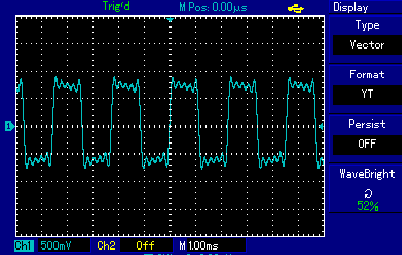
\includegraphics[width=10 cm, height = 7cm]{Rechteckspannung/3.png}
\end{figure}

\centerline{\textbf{Dreieckspannung}}
\begin{table}[H]
  \centering
  \begin{tabular}{c c}
    \toprule\\
    Anzahl & $a_n$ / V \\
    \midrule \\
    1 & 0,6204 \\
    3 & 0,0689 \\
    5 & 0,0248 \\
    7 & 0,0126 \\
    9 & 0,00076 \\
    \bottomrule
  \end{tabular}
  \caption{Darstellung der Amplitude zur Dreieckspannung}
  \label{tab:5}
\end{table}
\begin{figure}[H]
  \centering
	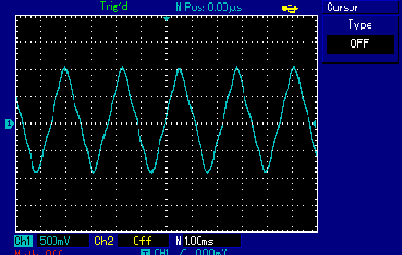
\includegraphics[width=10 cm , height=5cm]{Dreieckspannung/4.png}
\end{figure}
\centerline{\textbf{Sägezahnspannung}}
\begin{table}[H]
  \centering
  \begin{tabular}{c c}
    \toprule\\
    Anzahl & $b_n$ / V \\
    \midrule \\
    1 & 0,6204 \\
    2 & 0,3102 \\
    3 & 0,2068 \\
    4 & 0,1551 \\
    5 & 0,1240 \\
    6 & 0,1034 \\
    7 & 0,0886 \\
    8 & 0,0775 \\
    9 & 0,0689 \\
    \bottomrule
  \end{tabular}
  \caption{Darstellung der Amplitude zur Sägezahnspannung}
  \label{tab:6}
\end{table}
\begin{figure}[H]
  \centering
	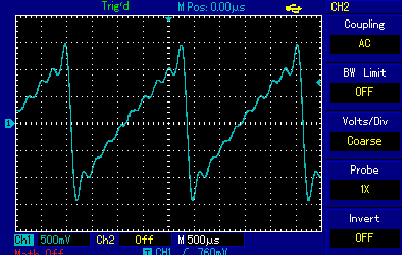
\includegraphics[width=10 cm , height=7cm]{Saegespannung/8.png}
\end{figure}
